\documentclass[12pt]{article}

\usepackage{palatino}
\usepackage{amsmath}
\usepackage{color}
\usepackage{graphicx}
\usepackage{epsfig}

% TexTalk Macros
\input textalk.tex
\input ../../TeX/newcom.tex
\input ../../TeX/symbols.tex

\textalktitle{Real-Time Motion Estimation for a Single Camera}{Andrew Davison}{March 2002}
\def\movie#1#2{\embedwide{#1}{#2.eps}{#2.mpg}} 

\advance\oddsidemargin by 15mm
\advance\textwidth by -30mm

% My general macros
\definecolor{brownbackcolour}{rgb}{0.29,0.21,0.0}
\definecolor{bluegreenbackcolour}{rgb}{0.17,0.27,0.26}
\definecolor{ajdyellowcolour}{rgb}{1.0,0.8,0.0}
\definecolor{ajdhighlightcolour}{rgb}{0.9,0.0,0.0}
\definecolor{ajdcobaltcolour}{rgb}{0.55,0.97,1.00}
\definecolor{ajddeepredcolour}{rgb}{0.30,0.07,0.05}
\definecolor{ajddeepbluecolour}{rgb}{0.11,0.20,0.24}
\def\ajdyellow#1{{\textcolor{ajdyellowcolour}{#1}}}
\def\brownback#1{{\textcolor{brownbackcolour}{#1}}}
\def\bluegreenback#1{{\textcolor{bluegreenbackcolour}{#1}}}
\def\ah#1{{\textcolor{ajdhighlightcolour}{#1}}}
\def\ajdcobalt#1{{\textcolor{ajdcobaltcolour}{#1}}}
\def\ajddeepred#1{{\textcolor{ajddeepredcolour}{#1}}}
\def\ajddeepblue#1{{\textcolor{ajddeepbluecolour}{#1}}}
\def\blue#1{{\textcolor{blue}{#1}}}
\def\black#1{{\textcolor{black}{#1}}}
\def\red#1{{\textcolor{red}{#1}}}
\def\yellow#1{{\textcolor{yellow}{#1}}}
\def\white#1{{\textcolor{white}{#1}}}


\setlength{\arrayrulewidth}{1mm} % Same as in \head
\setlength{\tabcolsep}{0.01\textwidth}

\newlength{\topspacer}
\setlength{\topspacer}{0.05\textheight}
\newlength{\tablespacer}
\setlength{\tablespacer}{0.05\textheight}




\def\ajdtitle#1{\centerline{\hugea \bf \sf  {#1}}}

%% \head
% A typical ``head of slide'' macro, but anything can be used.
% This one makes a table of contents entry
\renewcommand{\head}[1]{
%\clearpage
 \begin{center}~\\
 \huge\sf{#1}\\
\psfig{file=Figsajd/Bits/darkline.ps,width=\textwidth,height=15\px}
 \end{center}
 \usecounter{section}
 \addcontentsline{toc}{section}{\thepart\hspace{1em}#1}
}



\begin{document} \huge

\sf


%%%%%%%%%%%%%%%%%%%%%%%%%%%%%%%%% SLIDE

\clearpage
\begin{center}


\centerline{
\includegraphics[height=70\px]{Figsajd/Bits/empty.id}
}

{\hugea Real-Time Single Camera SLAM}\\[10mm]

\vspace{60\px}

\centerline{
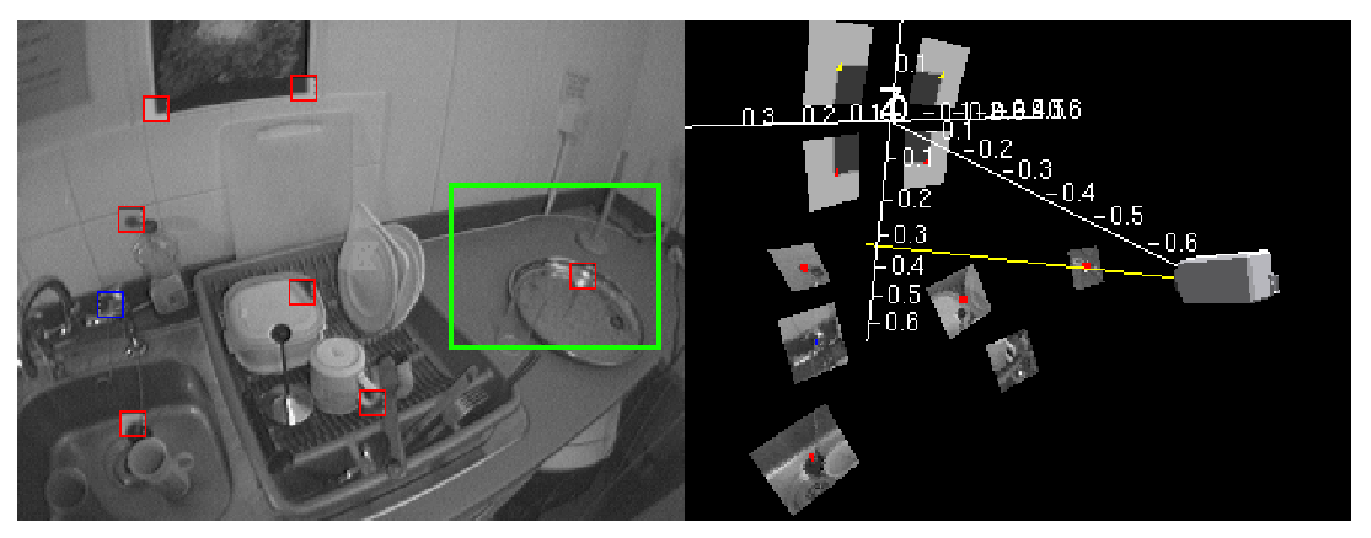
\includegraphics[height=220\px,clip]{Figsajd/Siggraph2004Results/planarpatches.eps}
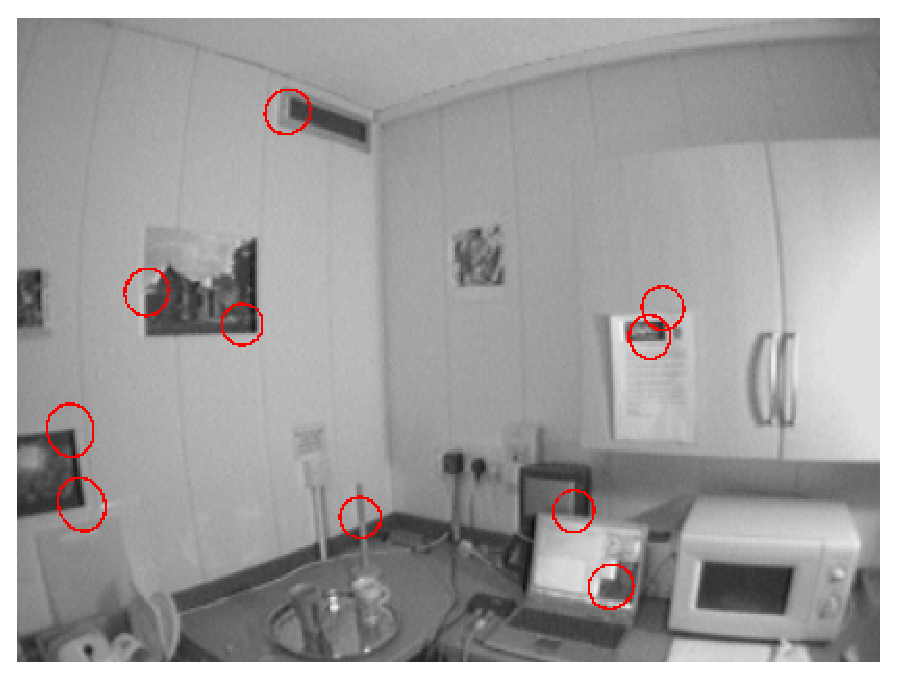
\includegraphics[height=220\px,clip]{Figsajd/Siggraph2004Results/activesearch.eps}
}


\vspace{80\px}


{\Large
\begin{tabular}{c}
{Andrew Davison}\\
{Department of Computing}\\
\end{tabular}
}

\vspace{2\px}
\centerline{

\includegraphics[width=210\px,clip]{Figsajd/Crest/imperial-logo-bigger.eps}
}




\vspace{5mm}



%%%%%%%%%%%%%%%%%%%%%%%%%%%%%%%%% SLIDE

\clearpage\head{The Ubiquitous Agile Camera}


\begin{tabular}{ccc}
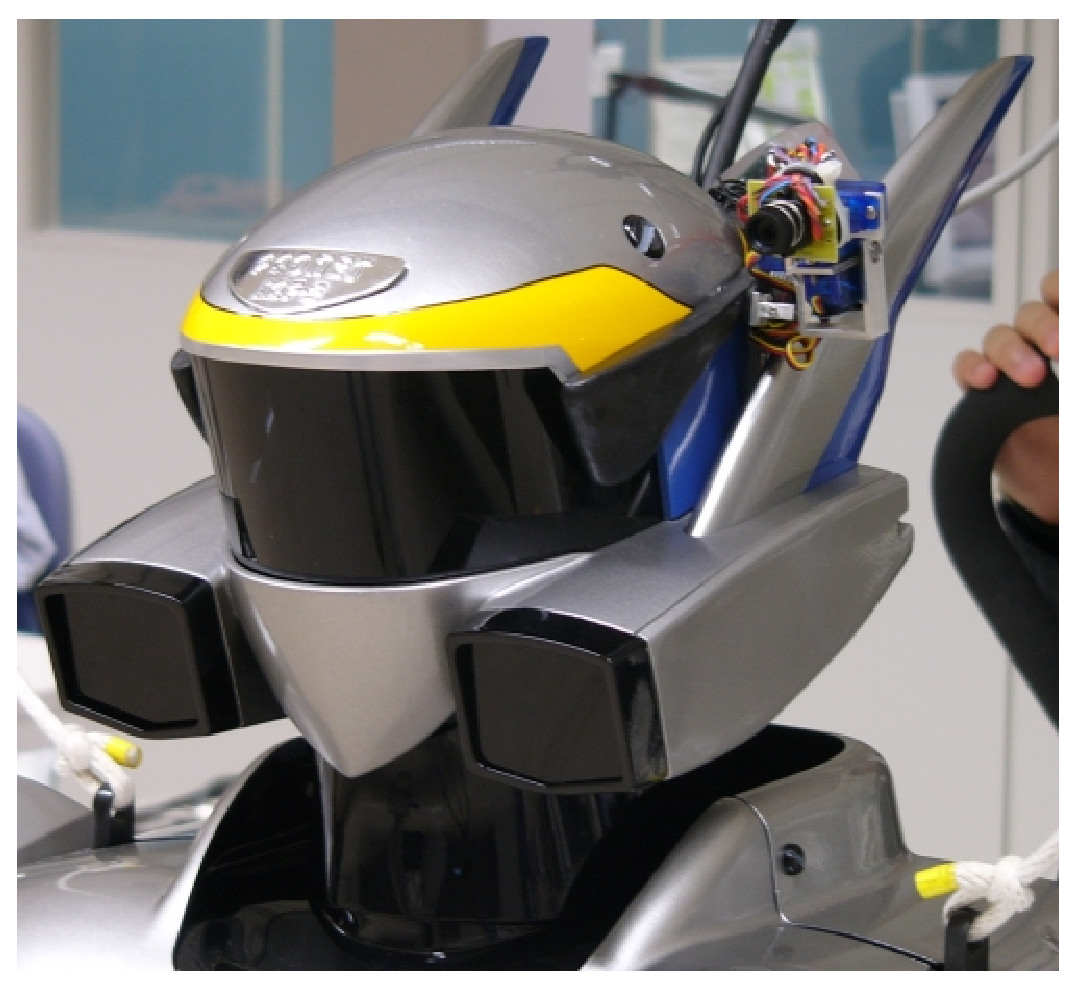
\psfig{file=Figsajd/Wearable/HRP-WeRo.eps,height=200\px}
&
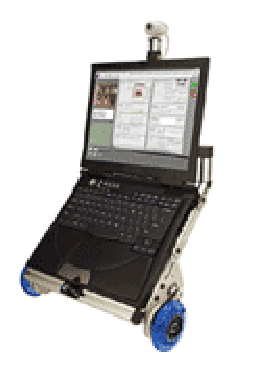
\psfig{file=Figsajd/MonoSLAMApp/er1.eps,height=200\px}
&
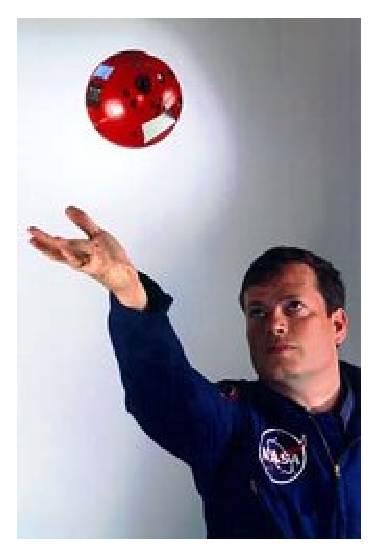
\psfig{file=Figsajd/MonoSLAMApp/nasa-psa.eps,height=200\px}
\\
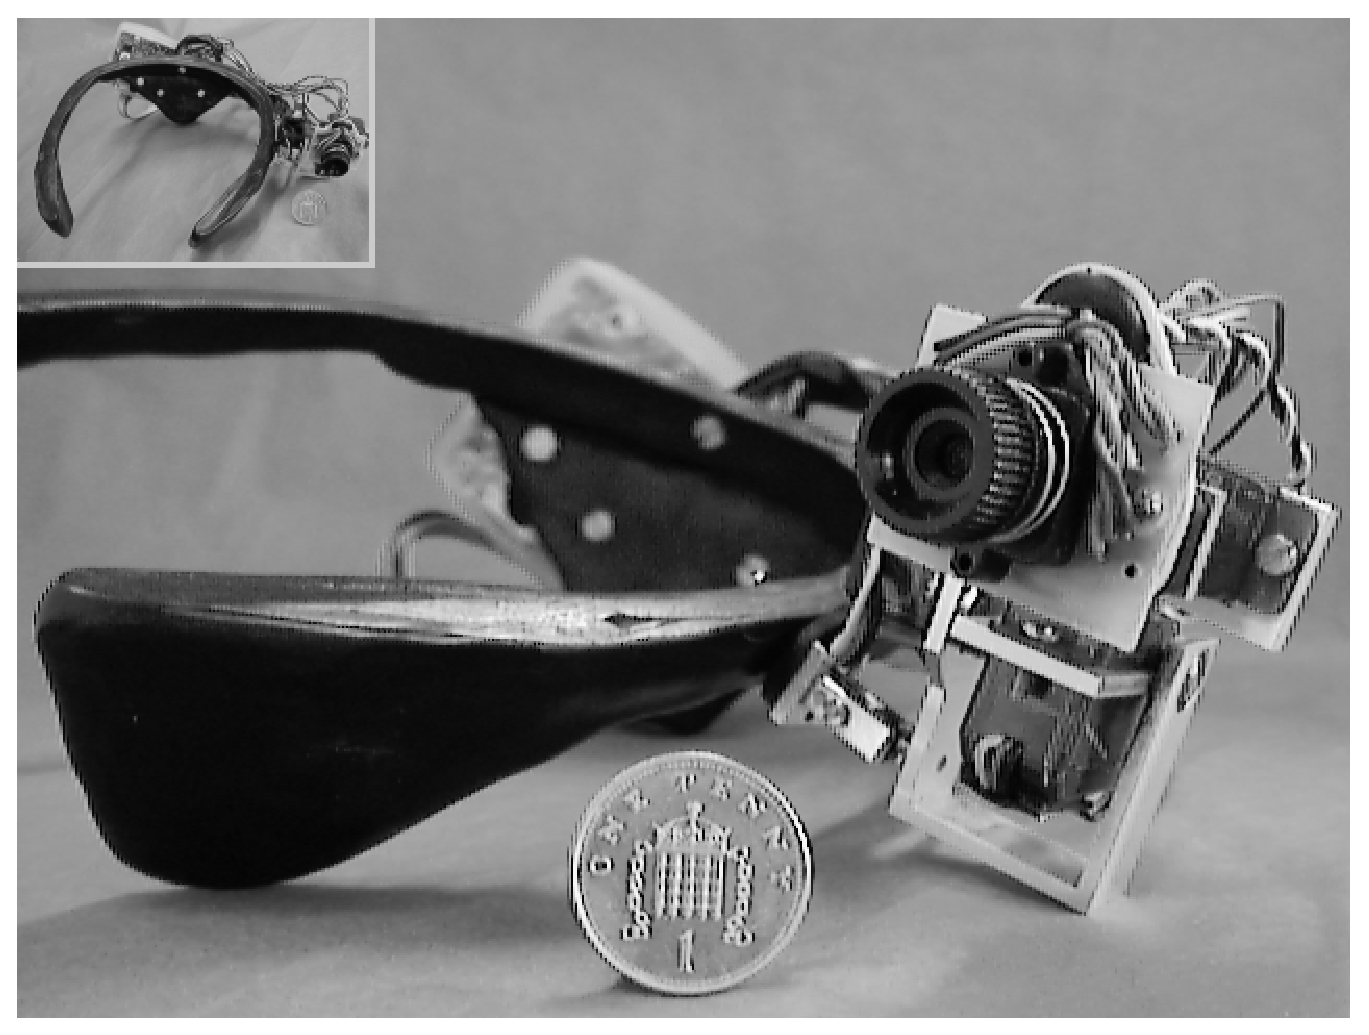
\psfig{file=Figsajd/Wearable/WeRoFW_combo.eps,height=200\px}
&
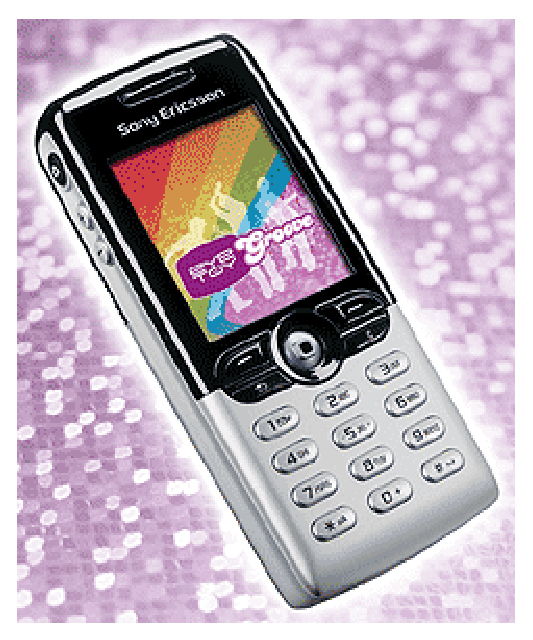
\psfig{file=Figsajd/MonoSLAMApp/sonyphone.eps,height=200\px}
&
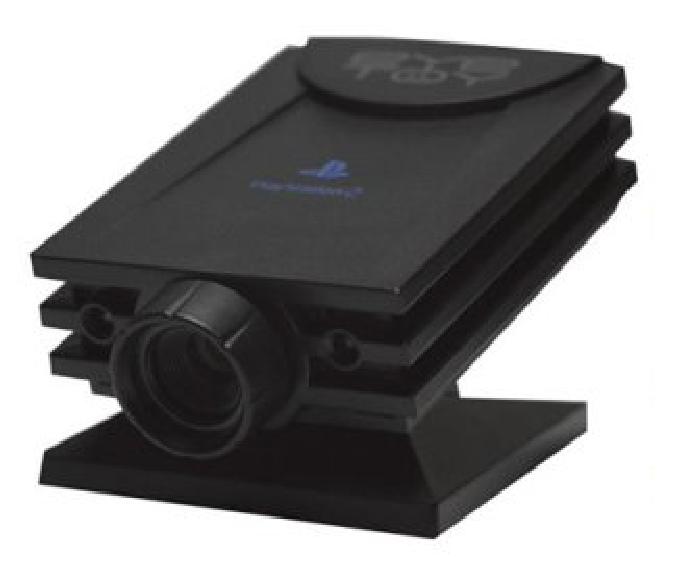
\psfig{file=Figsajd/MonoSLAMApp/eyetoy.eps,height=200\px}
\end{tabular}

Monocular video; unconstrained, high-acceleration, large-rotation motion.




%%%%%%%%%%%%%%%%%%%%%%%%%%%%%%%%% SLIDE

\clearpage
\head{Structure from Motion}


\vspace{-10mm}  

\bi
\item Historically derived from \ah{photogrammetry}
\item Projective geometry of a \ah{set of perspective images}
\item \ah{Uncalibrated} methods suitable for \ah{short sequence analysis}
\ei

\centerline{
\psfig{file=Figsajd/CameraGeom/essential.id,height=300\px}
}

\vspace{-50\px}





%%%%%%%%%%%%%%%%%%%%%%%%%%%%%%%%% SLIDE

\clearpage
\head{Structure from Motion}


\bi
\item An old example from Oxford's \ah{Visual Geometry Group} (Torr \& Zisserman)
\ei

\vspace{5mm}

\centerline{
\hfill
\awfembed{\psfig{file=Figsajd/Bits/empty.id,width=320\px,height=240\px}}{<embed type="video/x-mpeg" src="../Moviesajd/SLAMSchool/seq0-20.mpg" width="320" height="240"  autostart=yes loop=1 framerate="30">}
\hfill
\awfembed{\psfig{file=Figsajd/Bits/empty.id,width=320\px,height=240\px}}{<embed type="video/x-mpeg" src="../Moviesajd/SLAMSchool/structure.mpg" width="320" height="240"  autostart=yes loop=1 framerate="30">}
\hfill
}





%%%%%%%%%%%%%%%%%%%%%%%%%%%%%%%%% SLIDE

\clearpage
\head{Off-Line vs. Real-Time Processing}


\vspace{-20\px}
\ah{\huge Batch: Off-Line Processing}
\vspace{20\px}


\centerline{\hfill
\raisebox{0.2cm}{\psfig{file=Figsajd/SeqBatch/batchdata.id,width=4cm}} 
\raisebox{1.2cm}{\psfig{file=Figsajd/Bits/rightarrow.id,width=2cm}}
\colorbox{ajddeepbluecolour}{
\psfig{file=Figsajd/SeqBatch/batchres.id,width=3cm}
}
\hfill
}


\ah{\huge Sequential: Interactive Real-Time Processing}
\\
\vspace{10\px}


\centerline{
\colorbox{ajddeepbluecolour}{
\psfig{file=Figsajd/SeqBatch/seq1.id,width=3cm}
}
\raisebox{1.3cm}{\psfig{file=Figsajd/SeqBatch/seqdata.id,width=3cm}}
\colorbox{ajddeepbluecolour}{
\psfig{file=Figsajd/SeqBatch/seq2.id,width=3cm}
}
\raisebox{1.3cm}{\psfig{file=Figsajd/SeqBatch/seqdata.id,width=3cm}}
\colorbox{ajddeepbluecolour}{
\psfig{file=Figsajd/SeqBatch/seq3.id,width=3cm}
}
}










%%%%%%%%%%%%%%%%%%%%%%%%%%%%%%%%% SLIDE

\clearpage
\head{DROID, Harris \& Pike, AVC 1987}


\bi
\item ``\ah{Harris corner}'' matching in images
\item \ah{Independent Kalman Filter} per feature
\item Later parallel \ah{frame-rate} implementation
\ei

\vspace{5mm}

\centerline{
\hfill
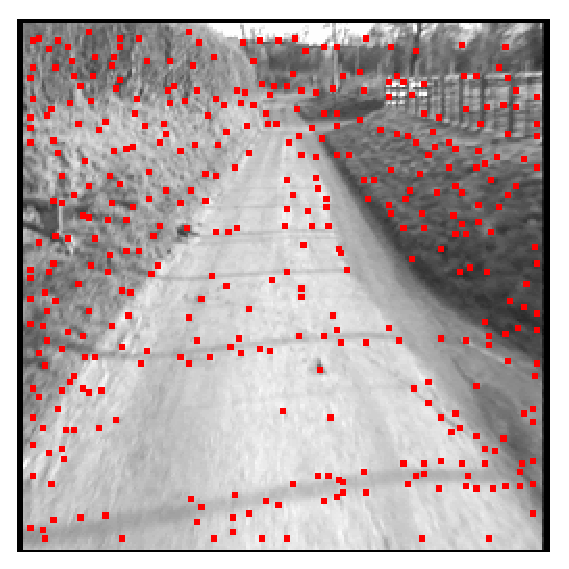
\psfig{file=Figsajd/SLAMSchool/droid_corners.eps,height=300\px}
\hfill
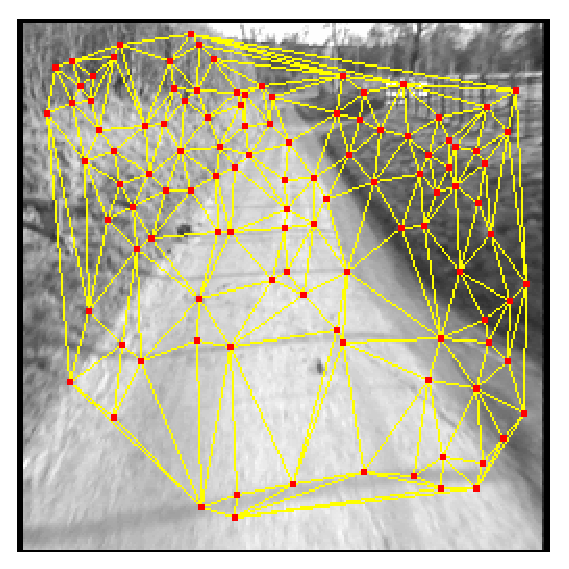
\psfig{file=Figsajd/SLAMSchool/droid_triangles.eps,height=300\px}
\hfill
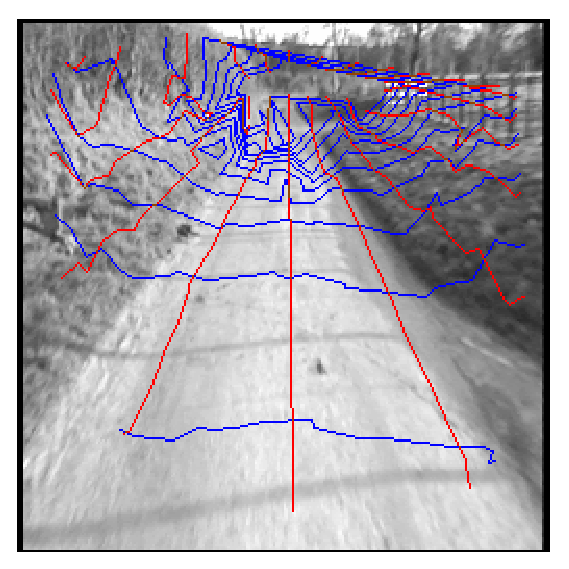
\psfig{file=Figsajd/SLAMSchool/droid_contours.eps,height=300\px}
\hfill
}





%%%%%%%%%%%%%%%%%%%%%%%%%%%%%%%%% SLIDE

\clearpage
\head{Visual Odometry, Nist\'{e}r et al., CVPR 2004}


\vspace{-5mm}  


\bi
\item \ah{Harris corner} matching
\item \ah{Pre-emptive RANSAC} to reject outliers
\item \ah{Monocular} or \ah{stereo}
\item \ah{Real-time frame-to-frame motion estimation}
\ei

\vspace{5mm}

\centerline{
\hfill
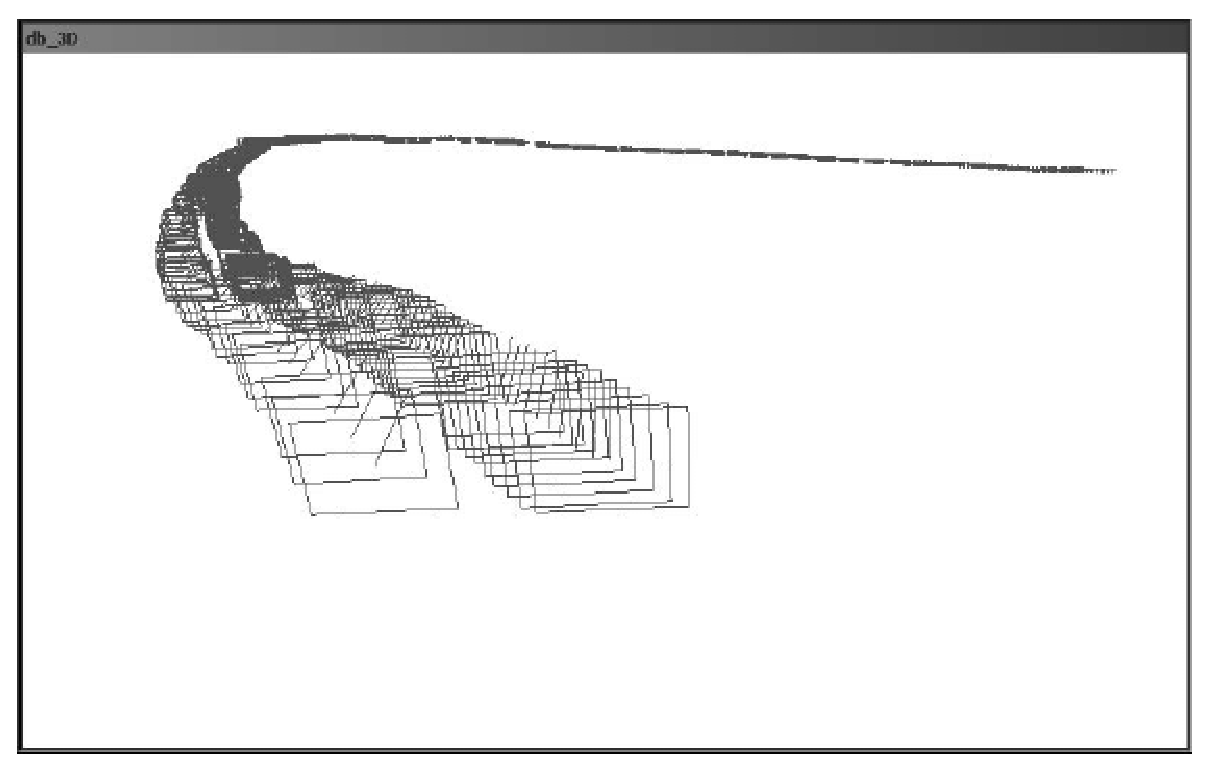
\psfig{file=Figsajd/SLAMSchool/nister_stereo.eps,height=300\px}
\hfill
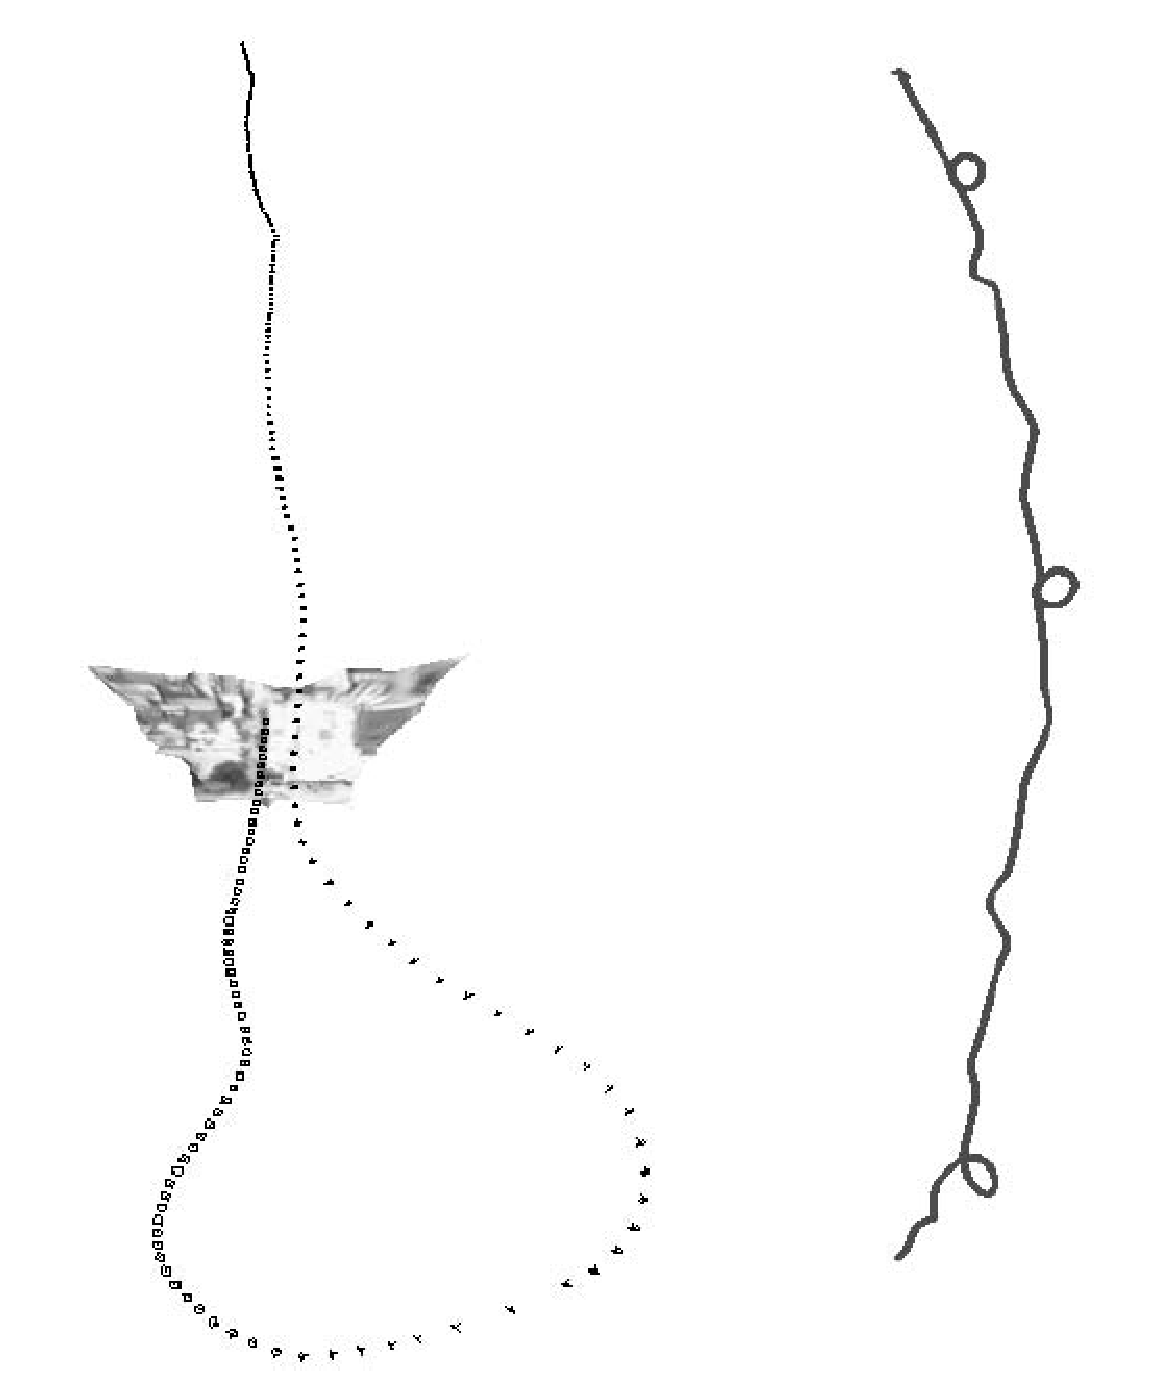
\psfig{file=Figsajd/SLAMSchool/nister_trajectories.eps,height=300\px}
\hfill
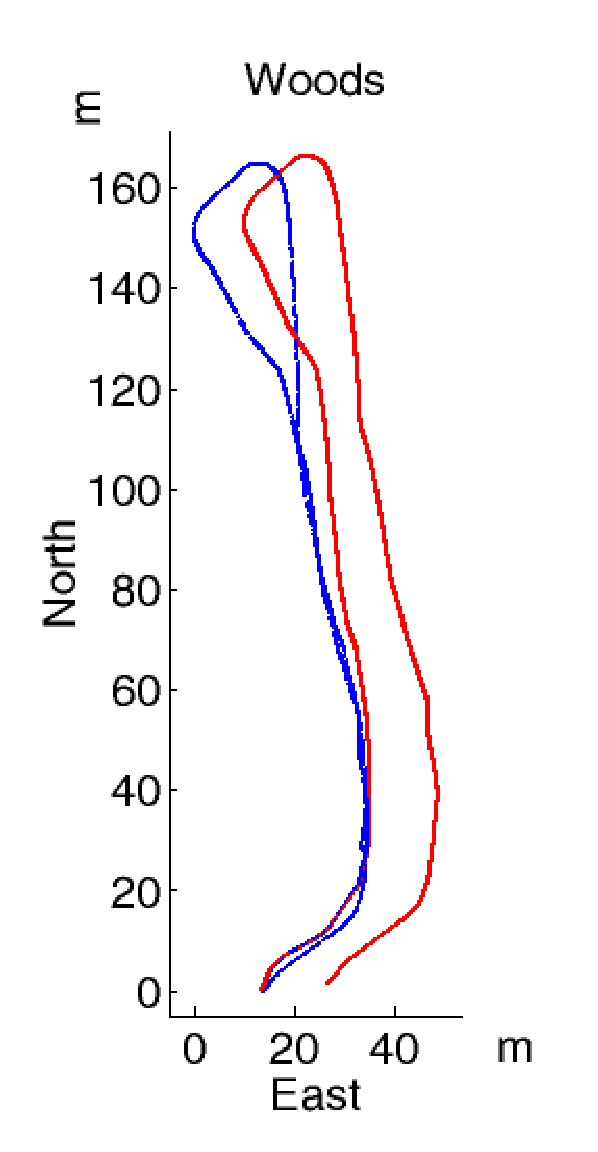
\psfig{file=Figsajd/SLAMSchool/nister_map.eps,height=300\px}
\hfill
}


%%%%%%%%%%%%%%%%%%%%%%%%%%%%%%%%% SLIDE

\clearpage\head{MonoSLAM, Davison ICCV 2003}


\vspace{-5mm}


\bi
\item 30Hz, \ah{full covariance SLAM}
\item ``\ah{Smooth motion}'' model
\item Prediction and \ah{guided search} for features
\item Features \ah{recaptured} after periods of neglect within room-sized environment
\ei

\vspace{3mm}


%%%%%%%%%%%%%%%%%%%%%%%%%%%%%%%%% SLIDE

\clearpage\head{MonoSLAM: Davison et al. 2003 \ldots}

\vspace{-4mm}

\centerline{
\awfembed{\psfig{file=Figsajd/Bits/empty.id,width=720\px,height=576\px}}{<embed type="video/x-mpeg" src="../Moviesajd/MonoSLAM/kitchen.mp4.avi" width="720" height="576"  autostart=yes loop=0 framerate="30">}
}

\vspace{-30mm}




%%%%%%%%%%%%%%%%%%%%%%%%%%%%%%%%% SLIDE

\clearpage\head{So Real-Time SFM is SLAM, but \ldots}

\vspace{-6mm}

\bi
\item In full 3D
\item With bearing-only measurement of visual features
(no direct distance measurement)
\item Usually with no odometry
\item At high frame-rates (30Hz +)
\ei

\ah{And often, in practical applications, with \ldots}

\bi
\item Repeated motion in a limited environment
\item An emphasis on real-time localisation
\item Sparse mapping
\ei


%%%%%%%%%%%%%%%%%%%%%%%%%%%%%%%%% SLIDE

\clearpage\head{What enables it to run in real-time?}


\vspace{-7mm}

\bi
\item Automatic \ah{sparse mapping} of high quality features
\item Motion modelling
\item \ah{Active search} guided by uncertainty.
\ei

\vspace{5mm}

{\Large
\begin{tabular}{|l|r|}
\hline
Image loading and administration &2ms\\
Image correlation searches &3ms\\
Kalman Filter update &5ms\\
Feature initialisation search &4ms\\
Graphical rendering &5ms\\
\hline
Total &19ms\\
\hline
\end{tabular}\\
}

\vspace{3mm}


30Hz processing on a notebook PC




%%%%%%%%%%%%%%%%%%%%%%%%%%%%%%%%% SLIDE

\clearpage\head{SLAM Using Active Vision}







\bi
\item Fixating active stereo measuring one feature at a time
\item 5Hz real-time processing (100MHz PC!)
\ei

\centerline{
\awfembed{\psfig{file=Figsajd/Bits/empty.id,width=384\px,height=288\px}}{<embed type="video/x-mpeg" src="../Moviesajd/GTI/move.mpg" width=384" height="288"  autostart=yes loop=1 framerate="15">}
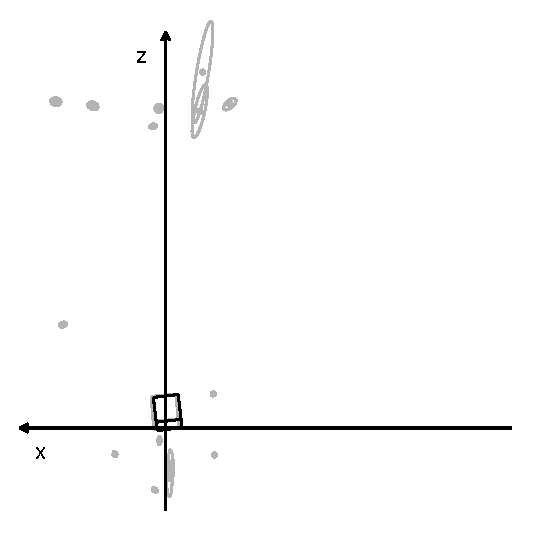
\psfig{file=Figsajd/GTI/run2.eps,height=288\px}
}

(Davison and Murray, ECCV 1998)




%%%%%%%%%%%%%%%%%%%%%%%%%%%%%%%%% SLIDE

\clearpage\head{Simultaneous Localisation and Mapping}


\ajdtitle{Propagating Probability Through Time}



\awfincludehtml{   <script language="javascript">}
% Split it to get newline that netscape seems to require in javascript
\awfincludehtml{
      i = 0; 
      images = new Array();
      images[0] = new Image;   images[0].src = "../Figsajd/SLAM/uc1.gif";
      images[1] = new Image;   images[1].src = "../Figsajd/SLAM/uc2.gif";
      images[2] = new Image;   images[2].src = "../Figsajd/SLAM/uc3.gif";
      images[3] = new Image;   images[3].src = "../Figsajd/SLAM/uc4.gif";
      images[4] = new Image;   images[4].src = "../Figsajd/SLAM/uc5.gif";
      images[5] = new Image;   images[5].src = "../Figsajd/SLAM/uc6.gif";
      images[6] = new Image;   images[6].src = "../Figsajd/SLAM/uc7.gif";
      function nextimage() {
          i++;
          if (i==7) {
              i=0;
          }
          document.theImage.src = images[i].src;
      }
    </script>
}


\awfincludehtml{<center><img src="transparent.gif" height=260 width=1><dt><img src="../Figsajd/SLAM/uc1.gif" name="theImage" width=587 height=458></center>}







%%%%%%%%%%%%%%%%%%%%%%%%%%%%%%%%% SLIDE

\clearpage\head{Simultaneous Localisation and Mapping}


\ajdtitle{First Order Uncertainty Propagation}


{\huge
\[
\vecxhat = \vecfour{\vecxhat_v}{\vecyhat_1}{\vecyhat_2}{\vdots} 
~~~~,~~~~
\matP = \matfour{\matP_{xx} & \matP_{xy_1} & \matP_{xy_2} & \ldots}
{\matP_{y_1x} & \matP_{y_1y_1} & \matP_{y_1y_2} & \ldots}
{\matP_{y_2x} & \matP_{y_2y_1} & \matP_{y_2y_2} & \ldots}
{\vdots       & \vdots         & \vdots         & }
\]
}


\bi
\item PDF over robot and map parameters is modelled as a single \ah{multi-variate Gaussian} and we can use the Extended Kalman Filter.
\ei



%%%%%%%%%%%%%%%%%%%%%%%%%%%%%%%%% SLIDE

\clearpage\head{MonoSLAM State Vector}


\vspace{-2mm}

Camera state representation: 3D \ah{position}, \ah{orientation}, \ah{velocity} and \ah{angular velocity:}

\vspace{-10mm}

\[
\vecx_v
~~ = ~~ 
\left(\begin{array}{l}\vecr^W\\\vecq^{WR}\\ \vecv^W \\ \vecomega^R \end{array}\right)
\]

\vspace{5mm}

Each feature state is a \ah{3D position vector}:

\vspace{-10mm}

\[
\vecy_i
~~ = ~~
\left(\begin{array}{l}x_i\\ y_i\\ z_i \end{array}\right)
\]



%%%%%%%%%%%%%%%%%%%%%%%%%%%%%%%%% SLIDE

\clearpage\head{Prediction Step: A Model for ``Smooth Motion''}


\vspace{-3mm}

\centerline{
\psfig{file=Figsajd/CameraGeom/smoothmotion.id,width=500\px}
}

``Constant \ah{velocity}, \ah{angular velocity}'' model $\Rightarrow$ bounded linear and angular acceleration

\vspace{-10mm}

\[
\vecf_v =
\left(\begin{array}{l}\vecr^W_{new}\\\vecq^{WR}_{new}\\ \vecv^W_{new} \\ \vecomega^R_{new} \end{array}\right)
=
\left(\begin{array}{l}\vecr^W + (\vecv^W + \vecV^W) \Delta t
\\\vecq^{WR} \times \vecq((\vecomega^R + \vecOmega^R) \Delta t)\\
\vecv^W + \vecV^W  \\ \vecomega^R + \vecOmega^R \end{array}\right)
\]




\vspace{-20mm}




%%%%%%%%%%%%%%%%%%%%%%%%%%%%%%%%% SLIDE

\clearpage\head{Measurement Step: Image Features and Active Search}


\centerline{
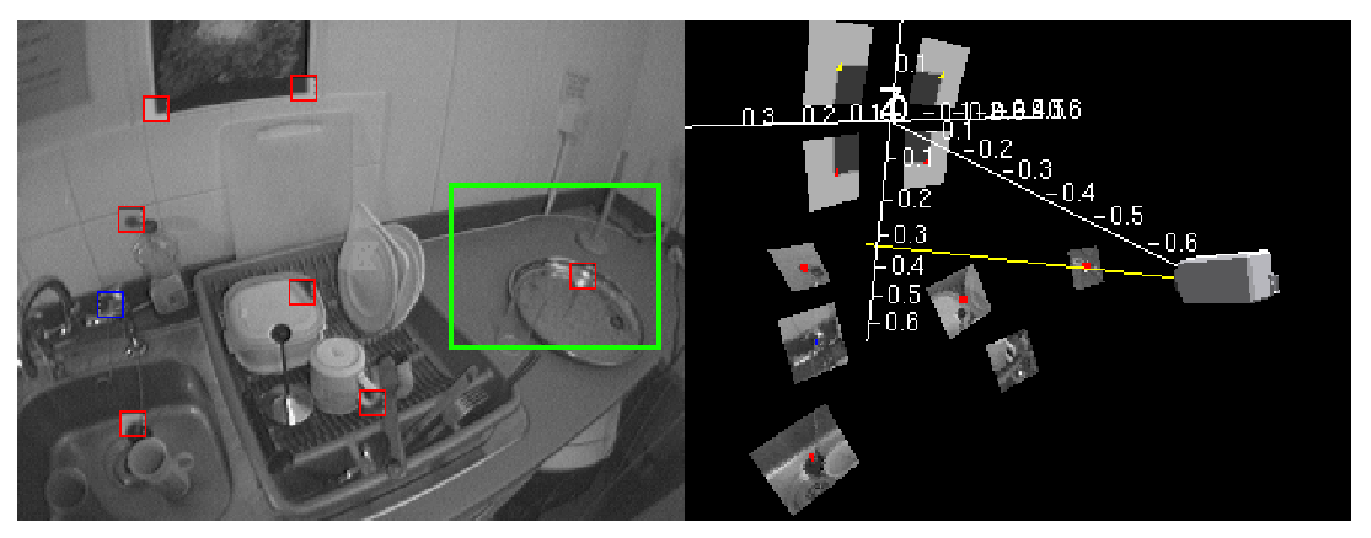
\epsfig{file=Figsajd/Siggraph2004Results/planarpatches.eps,height=220\px}
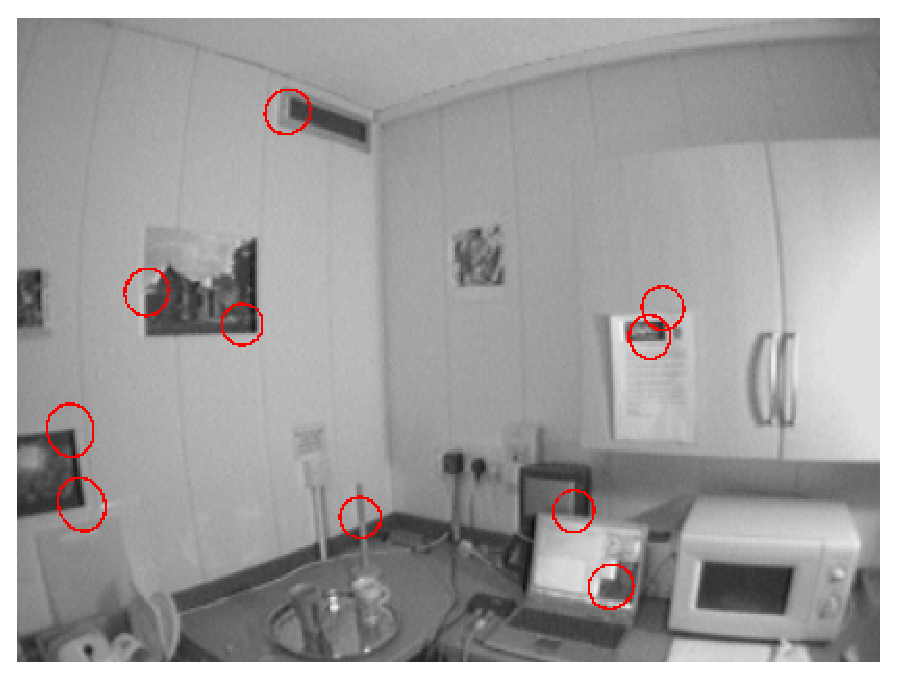
\epsfig{file=Figsajd/Siggraph2004Results/activesearch.eps,height=220\px}
}

\bi
\item \ah{Large salient feature patches} detected to serve as \ah{visual landmarks}.
\item Uncertainty-guided \ah{active search} within elliptical regions.
\ei


%%%%%%%%%%%%%%%%%%%%%%%%%%%%%%%%% SLIDE

\clearpage
\head{SLAM using SIFT, Se, Lowe, Little, ICRA 2001}


\vspace{-5mm}

\bi
\item \ah{SIFT} scale-invariant features
\ei

\vspace{5mm}

\centerline{
\hfill
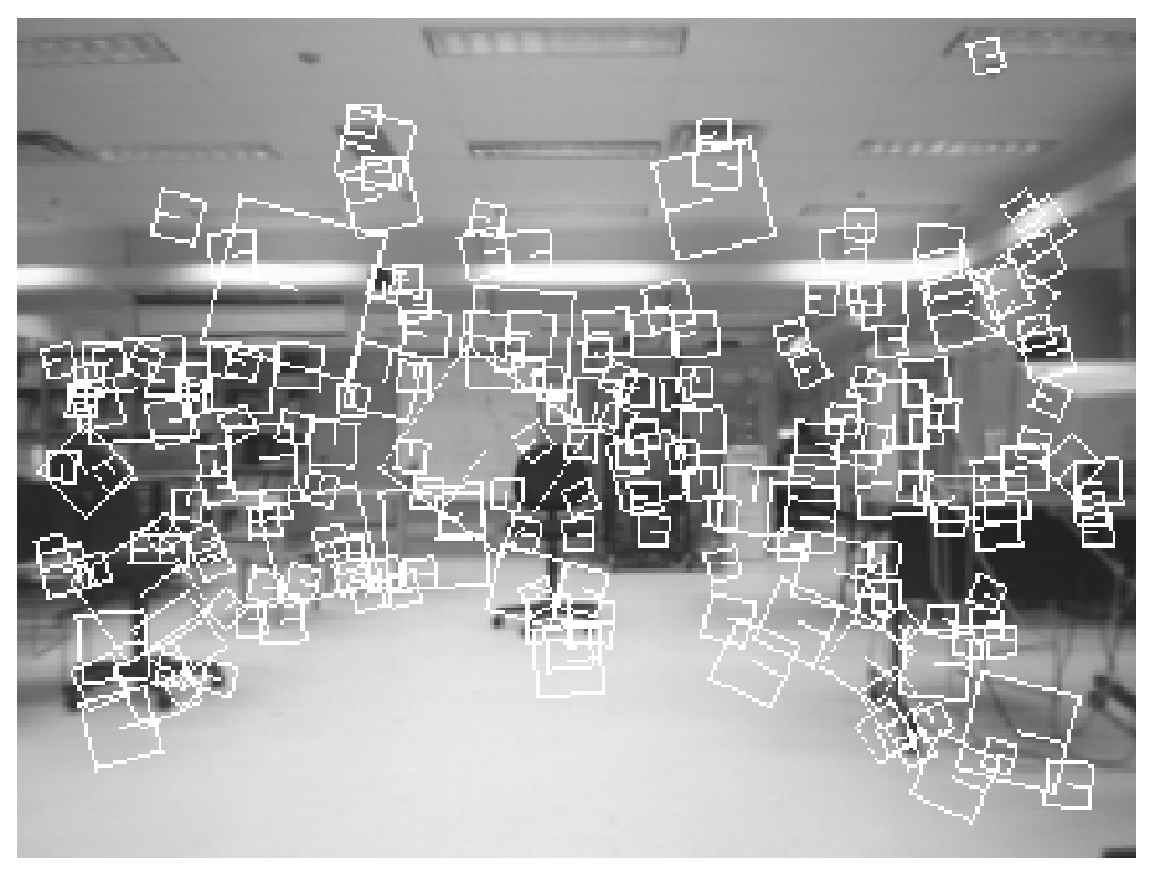
\psfig{file=Figsajd/SLAMSchool/se_sift.eps,height=320\px}
\hfill
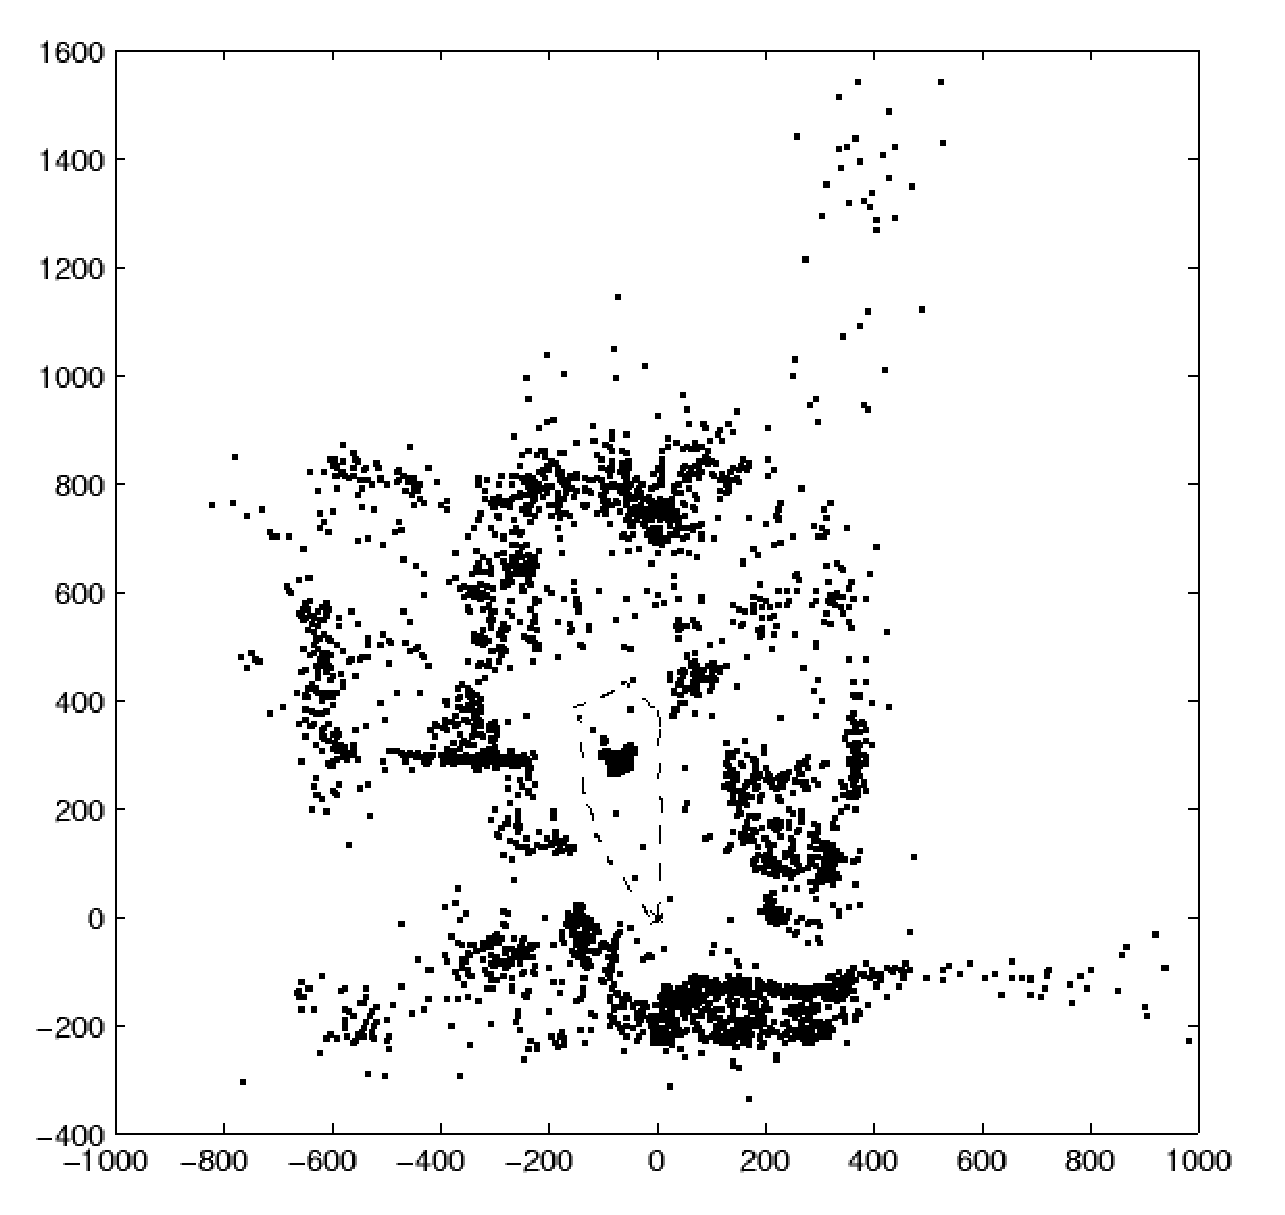
\psfig{file=Figsajd/SLAMSchool/se_map.eps,height=320\px}
\hfill
}



%%%%%%%%%%%%%%%%%%%%%%%%%%%%%%%%% SLIDE

\clearpage
\head{SIFT, David Lowe, UBC}


\vspace{-4mm}

\bi
\item \ah{SIFT} matches over whole image
\ei

\vspace{4mm}

\centerline{
\hfill
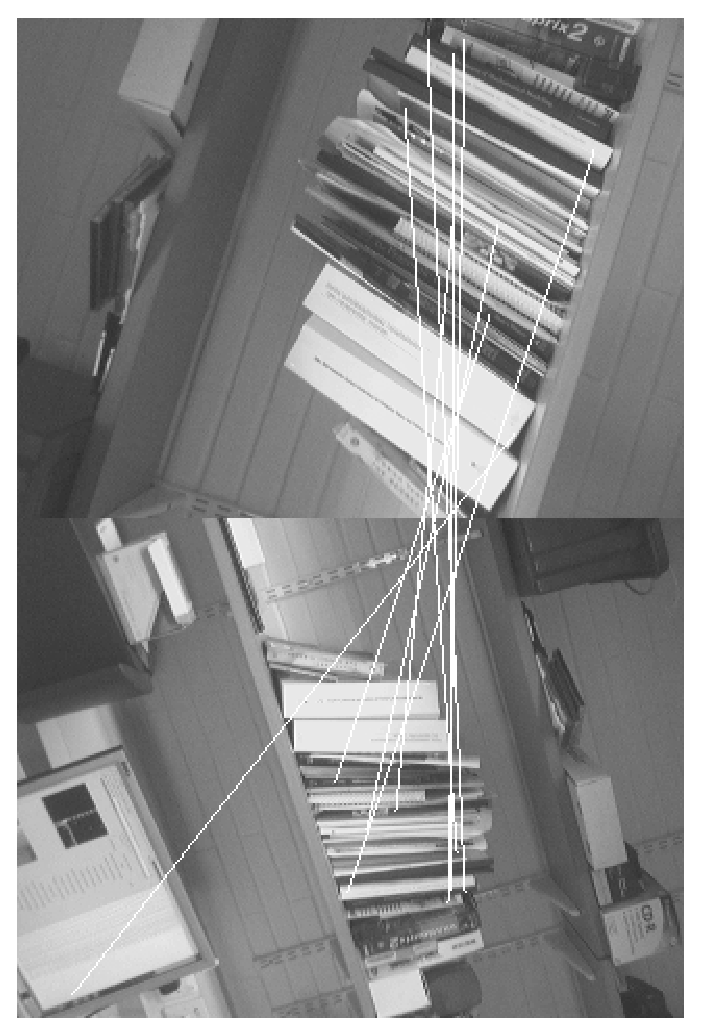
\psfig{file=Figsajd/SLAMSchool/sift_match1.eps,height=480\px}
\hfill
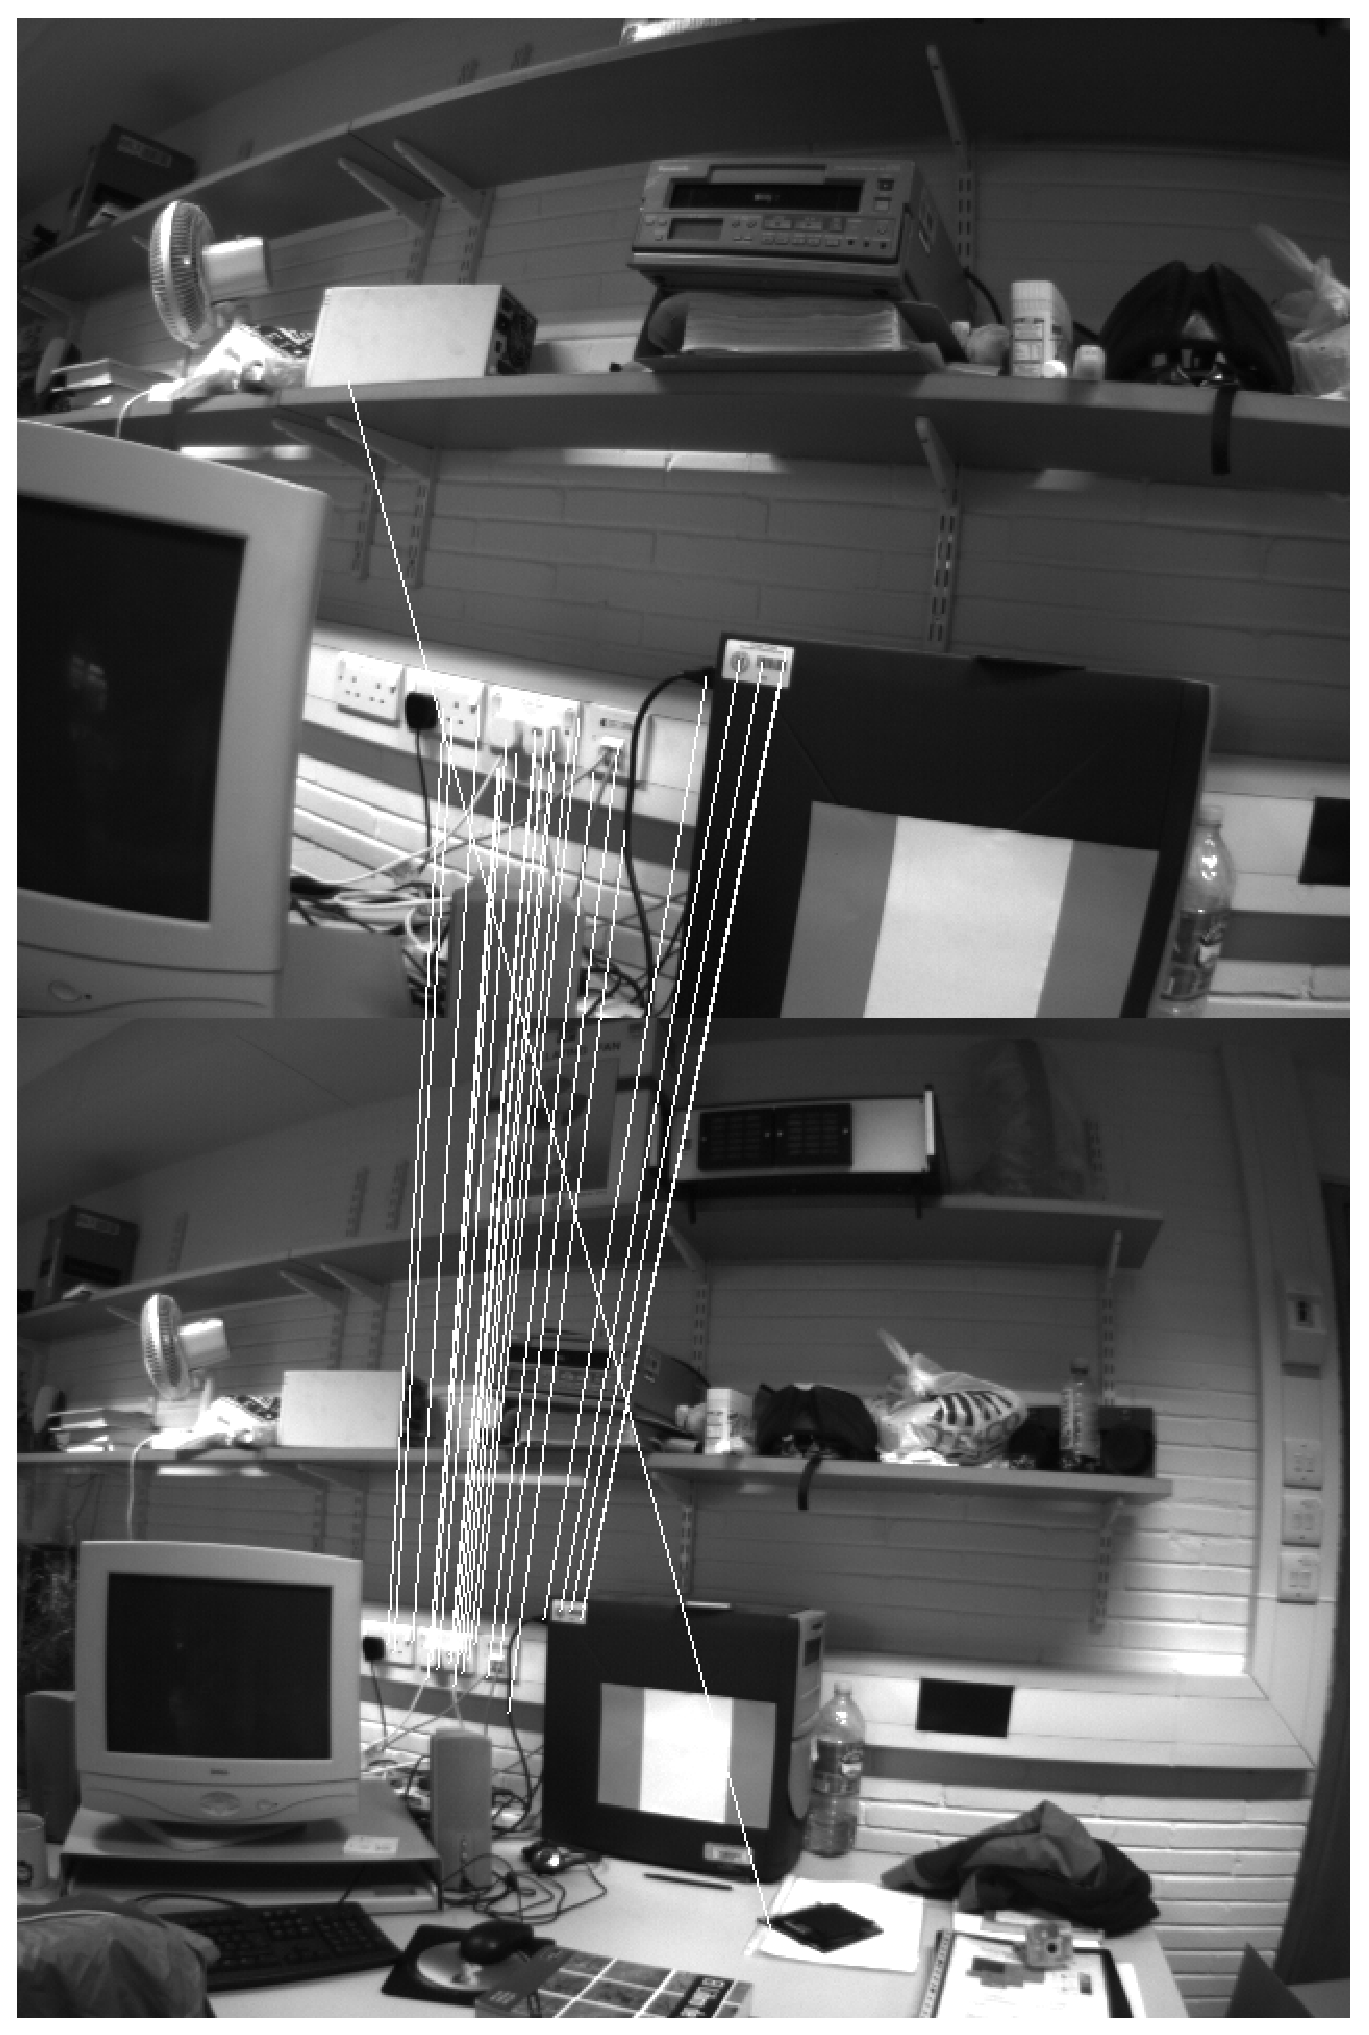
\psfig{file=Figsajd/SLAMSchool/sift_match2.eps,height=480\px}
\hfill
}



%%%%%%%%%%%%%%%%%%%%%%%%%%%%%%%%% SLIDE

\clearpage
\head{Vision-Based Exploration and Occupancy Mapping, Sim and Little IROS 2006}

\awfembed{\psfig{file=Figsajd/Bits/empty.id,width=350\px,height=350\px}}{<embed type="video/x-mpeg" src="../Moviesajd/SLAMSchool/simmapping.avi" width=350" height="350"  autostart=yes loop=no>}

\bi
\item SIFT features, FastSLAM, 1Hz updates
\item Dense occupancy mapping using stereo
\ei

%%%%%%%%%%%%%%%%%%%%%%%%%%%%%%%%% SLIDE

\clearpage\head{Active Search}

\ah{Priors} can tell us a lot:

\centerline{
\hfill
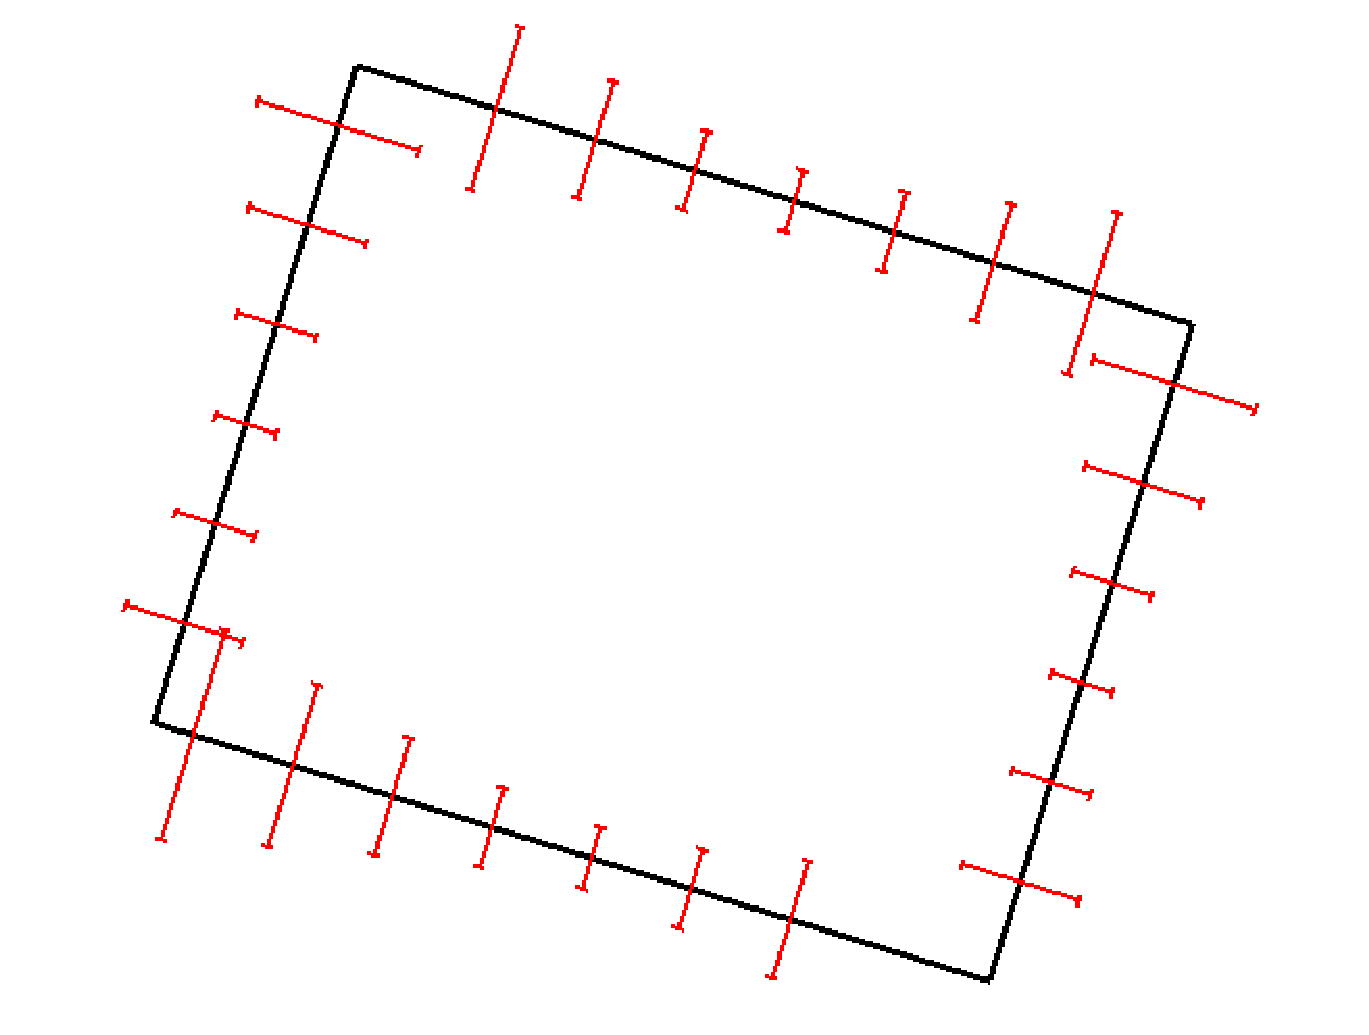
\psfig{file=Figsajd/ActiveSearch/edges_example.eps,width=320\px}
\hfill
}


\be
\item Where to look for the information we need
\item \ah{Expected utility} to the task at hand 
\item Likely \ah{computational effort} required
\ee

\ldots and even when we can stop.


%%%%%%%%%%%%%%%%%%%%%%%%%%%%%%%%% SLIDE

\clearpage\head{Probability and Entropy}

\vspace{-30\px}

\bi
\item Entropy of a \ah{discrete} statement set $x \in A_X$:
\ei

\vspace{-10\px}

\psfig{file=Figsajd/Probability/histogram.id,height=200\px}

\vspace{-40\px}

\[
H(X) = E\left[\log_2 \frac{1}{P(x)}\right]   = \sum_{x \in A_X} P(x) \log_2 \frac{1}{P(x)}
\]

\bi
\item \ah{Joint entropy}, in two or more variables:
\ei

\vspace{-30\px}

\[
H(XY) = E\left[\log_2 \frac{1}{P(xy)}\right]   
\]

%%%%%%%%%%%%%%%%%%%%%%%%%%%%%%%%% SLIDE

\clearpage\head{Mutual Information}

\bi
\item
\ah{Mutual Information (MI)} is the expected \\ \ah{reduction in entropy} of 
parameter on \\ learning the exact value of the other:
\ei

\vspace{-20\px}

\[
I(X;Y) = I(Y;X) = H(X) - H(X|Y)
\]

\vspace{30\px}

\bi
\item
In bit units, $I(X;Y)$ is \ah{how much information} we expect to 
learn about one
parameter by learning the value of the other.
\ei

%%%%%%%%%%%%%%%%%%%%%%%%%%%%%%%%% SLIDE

\clearpage\head{Continuous Probability Distributions}

\centerline{
\hfill
\psfig{file=Figsajd/Probability/histogram.id,height=160\px}
\hfill
\psfig{file=Figsajd/Bits/rightarrow.id,width=50\px,height=140\px}
\hfill
\psfig{file=Figsajd/Probability/histogram4.id,height=160\px}
\hfill
\psfig{file=Figsajd/Bits/rightarrow.id,width=50\px,height=140\px}
\hfill
\psfig{file=Figsajd/Probability/continuous.id,height=160\px}
\hfill
}


\vspace{-20 \px}

\[
H(X) = \sum_{x \in X} p(x) \delta x \log_2 \frac{1}{p(x) \delta x}
\]
\bi
\item As $\delta x \rightarrow 0$, entropy diverges, but mutual information remains well defined:
\ei
\[
I(X;Y) = \int_{x,y} p(x, y) \log_2 \frac{p(x|y)}{p(x)} dx dy
\]


%%%%%%%%%%%%%%%%%%%%%%%%%%%%%%%%% SLIDE

\clearpage\head{Multi-Variate Gaussian PDF}

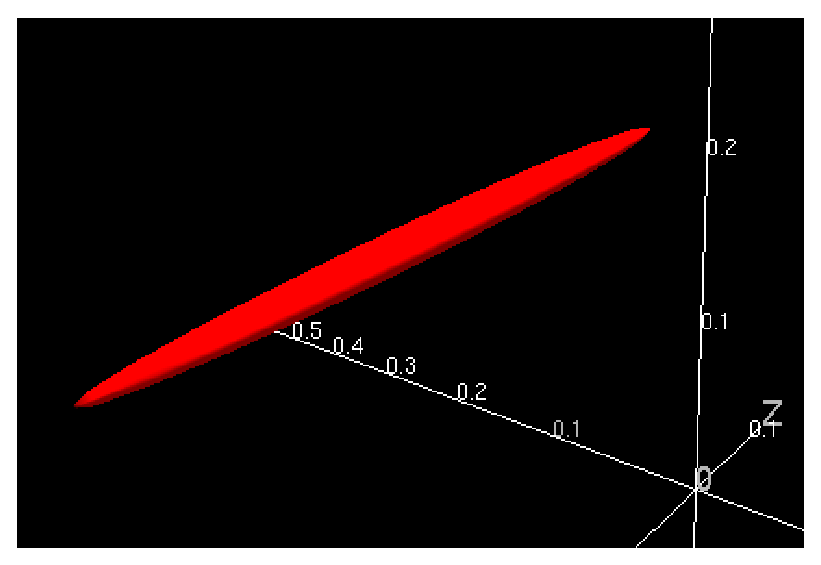
\psfig{file=Figsajd/ActiveSearch/ellipsoid.eps,width=400\px}


\bi
\item Represented in general by \ah{mean vector $\vecahat$} and \ah{covariance matrix $\matP_{aa}$}:
\ei

\vspace{-20\px}

\[
p(\veca) = (2 \pi)^{-\frac{N}{2}} |\matP_{aa}|^{-\frac{1}{2}} e^{-\frac{1}{2}(\veca - \vecahat)^\top \matP_{aa}^{-1}(\veca - \vecahat)} 
\]


%%%%%%%%%%%%%%%%%%%%%%%%%%%%%%%%% SLIDE

\clearpage\head{MI of a Multi-Variate Gaussian PDF}



\bi
\item 
We divide $\veca$ into \ah{two partitions $\vecalpha$ and $\vecbeta$}:
\ei
\[
\vecahat = \vectwo{\vecalphahat}{\vecbetahat} ~; ~ \matP_{aa} = \mattwo{\matP_{\alpha\alpha}}{\matP_{\alpha\beta}}{\matP_{\beta\alpha}}{\matP_{\beta\beta}}
\]

\bi
\item And apply the \ah{general rule for conditioning}:
\ei
\bea
\vecalphahat' &=& \vecalphahat + \matP_{\alpha\beta}
\matP_{\beta\beta}^{-1} (\vecbeta - \vecbetahat) \label{eqn:vecalpha} \nonumber\\
\matP_{\alpha\alpha}' &=& \matP_{\alpha\alpha} -
\matP_{\alpha\beta} \matP_{\beta\beta}^{-1} \matP_{\beta\alpha} \nonumber
\label{eqn:Palpha}
\eea



%%%%%%%%%%%%%%%%%%%%%%%%%%%%%%%%% SLIDE

\clearpage\head{MI of a Multi-Variate Gaussian PDF}


\bi
\item To derive the \ah{mutual information} of partitions $\vecalpha$~and~$\vecbeta$:
\ei
\[
I(\vecalpha; \vecbeta) =
\frac{1}{2} \log_2 \frac{  |\matP_{\alpha\alpha}| }
{|\matP_{\alpha\alpha} -
\matP_{\alpha\beta} \matP_{\beta\beta}^{-1} \matP_{\beta\alpha}|} 
\]


\bi
\item Davison, ICCV 2005
\ei


%%%%%%%%%%%%%%%%%%%%%%%%%%%%%%%%% SLIDE


\clearpage\head{Feature Search in Model-Based Tracking}

\vspace{-25\px}

\bi
\item Object state \ah{$\vecx$} and measurement candidates \ah{$\vecz_i = \vech_i(\vecx) + \vecn_m$}
\ei

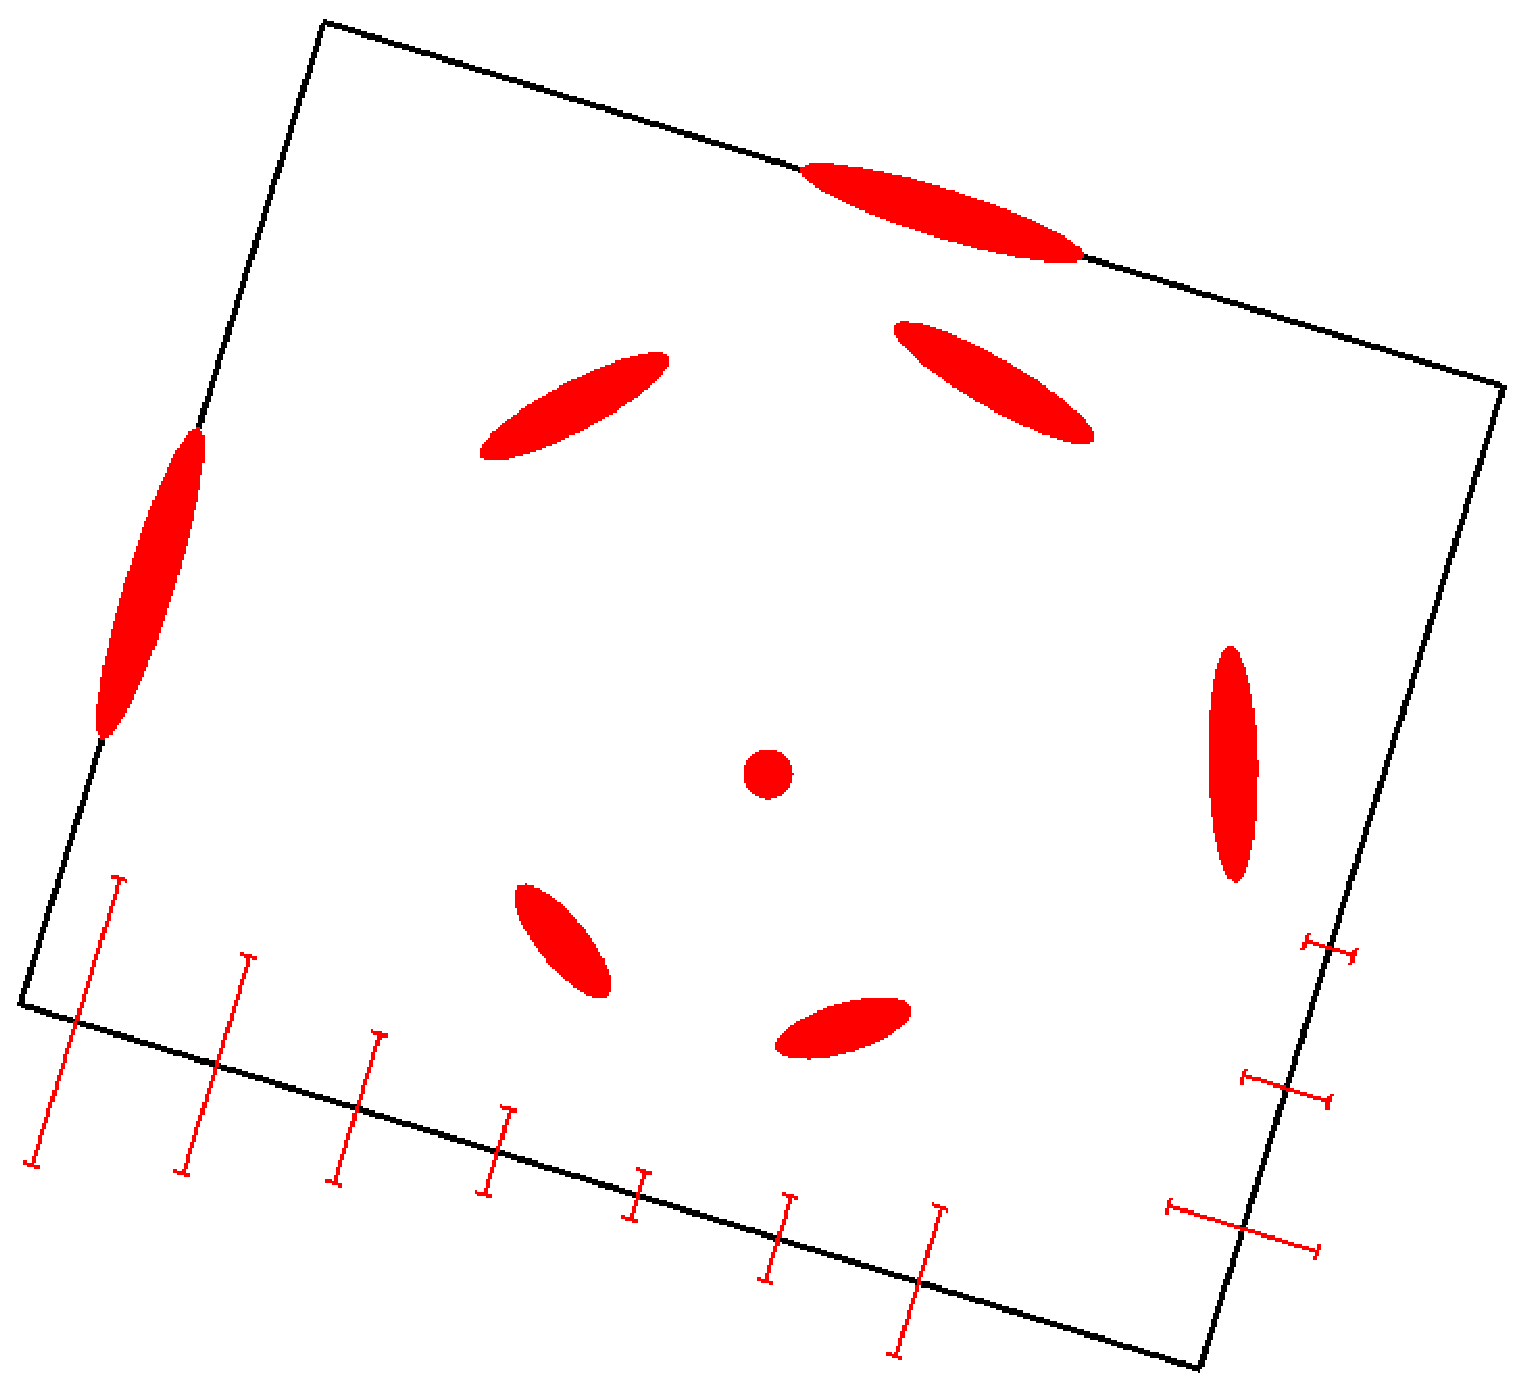
\psfig{file=Figsajd/ActiveSearch/example1.eps,width=270\px}

\vspace{-25\px}

{\Large
\[
\vecxhat_m = \vecfour{\vecxhat}{\veczhat_1}{\veczhat_2}{\vdots} ~,~
\matP_{\vecx_m} = \matfour
{\matP_x & \matP_x \pdiff{\vech_1}{\vecx}^\top &
\matP_x \pdiff{\vech_2}{\vecx}^\top & \ldots  }
{\pdiff{\vech_1}{\vecx} \matP_x & \pdiff{\vech_1}{\vecx} \matP_x
\pdiff{\vech_1}{\vecx}^\top + \matR_1 & \pdiff{\vech_1}{\vecx} \matP_x
\pdiff{\vech_2}{\vecx}^\top & \ldots}
{\pdiff{\vech_2}{\vecx} \matP_x & \pdiff{\vech_2}{\vecx} \matP_x
\pdiff{\vech_1}{\vecx}^\top & \pdiff{\vech_2}{\vecx} \matP_x
\pdiff{\vech_2}{\vecx}^\top + \matR_2 & \ldots}
{\vdots & \vdots & \vdots &}
\]
}

\vspace{-200\px}

%%%%%%%%%%%%%%%%%%%%%%%%%%%%%%%%% SLIDE


\clearpage\head{Measurement Information Matrix}

\[
\matI(\vecx_m) = \matfour{* & I(\vecx; \vecz_1) & I(\vecx; \vecz_2)
& \ldots}
{I(\vecz_1; \vecx) & * & I(\vecz_1; \vecz_2) & \ldots}
{I(\vecz_2; \vecx) & I(\vecz_2; \vecz_1) & * & \ldots}
{\vdots & \vdots & \vdots & }
\]

\bi
\item MI between each measurement and state
\item MI between each pair of measurements
\ei

%%%%%%%%%%%%%%%%%%%%%%%%%%%%%%%%% SLIDE


\clearpage\head{Tracking a Translating, Rotating Object in 2D}


\includegraphics[width=320\px,clip]{Figsajd/ActiveSearch/twodtrack.id}

\vspace{-30\px}

{\Large
\[
\vecxhat = \vecthree{u}{v}{\phi} = \vecthree{320.0}{260.0}{0.3} ~,~ 
\vecP_x =\matthreeright
{7.0 }{	0.0 }{	0.0}
{0.0 }{	7.0 }{	0.0}
{0.0 }{	0.0 }{	0.007} ~.
\label{eqn:statecov}
\]
}

\vspace{-30\px}


\bi
\item 2D \ah{point feature} measurements
\item 1D \ah{edge feature} measurement
\item One pixel measurement uncertainty 
\ei

%%%%%%%%%%%%%%%%%%%%%%%%%%%%%%%%% SLIDE

\clearpage\head{Information-Guided Search with Point Features}

\awfembed{\psfig{file=Figsajd/Bits/empty.id,width=480\px,height=360\px}}{<a href="dummy.activesearchpoints">
<img src="../Figsajd/ActiveSearch/points_example.jpg" border=0 width=480 height=360></a>}


\bi
\item Reasonable estimation with 2 well-chosen measurements
\ei

%%%%%%%%%%%%%%%%%%%%%%%%%%%%%%%%% SLIDE

\clearpage\head{Information-Guided Search with Edge Features}

\awfembed{\psfig{file=Figsajd/Bits/empty.id,width=480\px,height=360\px}}{<a href="dummy.activesearchedgespoints">
<img src="../Figsajd/ActiveSearch/edges_points_example.jpg" border=0 width=480 height=360></a>}

\bi
\item Reasonable estimation with 3 well-chosen measurements
\ei



%%%%%%%%%%%%%%%%%%%%%%%%%%%%%%%%% SLIDE

\clearpage\head{The Cost of Image Processing}

\bi
\item Cost of point feature search proportional to ellipse area
$A = \pi N_\sigma^2
\sqrt{|\matP_i|}$
\item Cost of edge feature search proportional to search line length
$L = 2 N_\sigma \sqrt{|\matP_i|}$
\ei

\ah{
Information efficiency $= \frac{\mbox{mutual information}}{\mbox{computational cost}}$
}

\bi
\item
To compare efficiency of different \\measurement types we need to
evaluate \\constants of proportionality 
\ei


%%%%%%%%%%%%%%%%%%%%%%%%%%%%%%%%% SLIDE

\clearpage\head{Search Guided by Information Efficiency}

\awfembed{\psfig{file=Figsajd/Bits/empty.id,width=480\px,height=360\px}}{<a href="dummy.activesearchpoints">
<img src="../Figsajd/ActiveSearch/costs_example.jpg" border=0 width=480 height=360></a>}

\vspace{-30\px}

\bi
\item Assume image processing is dominant \\computational cost
\item Same level of accuracy obtained with around 700 correlation operations rather than 1900
\ei




%%%%%%%%%%%%%%%%%%%%%%%%%%%%%%%%% SLIDE

\clearpage\head{SLAM with Lines (Smith et al. BMVC 2006)}

\awfembed{\psfig{file=Figsajd/Bits/empty.id,width=820\px,height=460\px}}{<embed type="video/x-mpeg" src="../Moviesajd/SLAMLines/office.avi" width=820" height="460"  autostart=yes loop=no>}

(Also approaches by Eade and Drummond (BMVC 2006), Lemaire et al., Gee et al.)



%%%%%%%%%%%%%%%%%%%%%%%%%%%%%%%%% SLIDE

\clearpage\head{Monocular Feature Initialisation}


\centerline{
\psfig{file=Figsajd/ICCV2003Results/init1.ps,width=300\px}
\psfig{file=Figsajd/ICCV2003Results/init2.ps,width=300\px}
\psfig{file=Figsajd/ICCV2003Results/init3.ps,width=300\px}
}
\centerline{
\psfig{file=Figsajd/ICCV2003Results/init4.ps,width=300\px}
\psfig{file=Figsajd/ICCV2003Results/init5.ps,width=300\px}
\psfig{file=Figsajd/ICCV2003Results/depthplot2.eps,width=300\px}
}

Particle (histogram) method, Davison ICCV 2003

%%%%%%%%%%%%%%%%%%%%%%%%%%%%%%%%% SLIDE

\clearpage\head{Low Parallax Binocular Reconstruction}

\epsfig{file=Figsajd/Monti/xz_vs_lambda_theta_gimped.eps,width=700\px}

\bi
\item Monte Carlo simulation reveals high Gaussianity in $\rho, \theta$ space where $\rho$ is {\em inverse depth}
\ei


%%%%%%%%%%%%%%%%%%%%%%%%%%%%%%%%% SLIDE

\clearpage\head{Unified Inverse Depth Parameterisation for Monocular SLAM}

A scene 3D point $i$ is defined by the state vector:
\[
\vecy_i=\left(\begin{array}{cccccc}x_i & y_i & z_i & \theta_i &
\phi_i & \rho_i\end{array}\right)^\top
\]
which models a 3D point located at:
\[
\left(\begin{array}{c}x_i\\y_i\\z_i\end{array}\right)+
                    \frac{1}{\rho_i}\vecm\left(\theta_i,
                    \phi_i\right)
\]




\bi
\item Montiel, Civera, Davison, RSS 2006
\ei


%%%%%%%%%%%%%%%%%%%%%%%%%%%%%%%%% SLIDE



\awfembed{\psfig{file=Figsajd/Bits/empty.id,width=720\px,height=720\px}}{<embed type="video/x-mpeg" src="../Moviesajd/Monti/juslibol_SLAM.mpg" width="720" height="720"  autostart=yes loop=0 framerate="30">}




%%%%%%%%%%%%%%%%%%%%%%%%%%%%%%%%% SLIDE

\clearpage\head{Loop Closing Using Inverse Depth Parameterisation}

\awfembed{\psfig{file=Figsajd/Bits/empty.id,width=640\px,height=240\px}}{<embed type="video/x-mpeg" src="../Moviesajd/Monti/cerradoDeBucle.avi" width="640" height="240"  autostart=yes loop=0 framerate="30">}



%%%%%%%%%%%%%%%%%%%%%%%%%%%%%%%%% SLIDE

\clearpage\head{SLAM with Infinite Points: a 30Hz Visual Compass}



\awfembed{\psfig{file=Figsajd/Bits/empty.id,width=640\px,height=240\px}}{<a href="dummy.monoslaminfiniteglowrealtime">
<img src="../Figsajd/PureRotation/rah_example.jpg" border=0 width=640 height=240></a>}


\bi
\item Montiel and Davison ICRA 2006
\item All features assumed to be at infinity: rotating camera
\ei


%%%%%%%%%%%%%%%%%%%%%%%%%%%%%%%%% SLIDE

\clearpage\head{Consistent Real-time Mosaicing}

\awfembed{\psfig{file=Figsajd/Bits/empty.id,width=579\px,height=241\px}}{<embed type="video/x-mpeg" src="../Moviesajd/Monti/alberthallmosaic.avi" width="579" height="241"  autostart=no loop=1 framerate="30">}


\bi
\item Real-time mosaic generation
\ei




%%%%%%%%%%%%%%%%%%%%%%%%%%%%%%%%% SLIDE

\clearpage\head{FastSLAM-Based Monocular SLAM}


\awfembed{\psfig{file=Figsajd/Bits/empty.id,width=800\px,height=338\px}}{<embed type="video/x-mpeg" src="../Moviesajd/SLAMSchool/eadedrummondslam.mpg" width="800" height="338"  autostart=yes loop=0 framerate="30">}

Eade and Drummond, CVPR 2006




%%%%%%%%%%%%%%%%%%%%%%%%%%%%%%%%% SLIDE
\clearpage\head{MonoSLAM in Medical Inspection / MIS}


\awfembed{\psfig{file=Figsajd/Bits/empty.id,width=568\px,height=464\px}}{<embed type="video/x-mpeg" src="../Moviesajd/MIS/bronchialimage.avi" width="568" height="464"  autostart=yes loop=0 framerate="30">}


Mountney, Stoyanov, Davison, Yang, MICCAI 2006

%%%%%%%%%%%%%%%%%%%%%%%%%%%%%%%%% SLIDE
\clearpage\head{MonoSLAM in Medical Inspection / MIS}


\awfembed{\psfig{file=Figsajd/Bits/empty.id,width=568\px,height=467\px}}{<embed type="video/x-mpeg" src="../Moviesajd/MIS/bronchial3d.avi" width="568" height="467"  autostart=yes loop=1 framerate="30">}


Mountney, Stoyanov, Davison, Yang, MICCAI 2006

%%%%%%%%%%%%%%%%%%%%%%%%%%%%%%%%% SLIDE
\clearpage\head{HRP2 Humanoid from AIST, Japan}


\vspace{5mm}




\centerline{
\awfembed{\psfig{file=Figsajd/Bits/empty.id,width=352\px,height=240\px}}{<embed type="video/x-mpeg" src="../Moviesajd/HRP/CircleHRP2.mpg" width=352" height="240"  autostart=yes loop=1 framerate="30">}
}

\bi
\item Small circular loop within a large room
\item No re-observation of `old' features until \\closing of large loop.
\ei



%%%%%%%%%%%%%%%%%%%%%%%%%%%%%%%%% SLIDE
\clearpage\head{HRP2 Loop Closure}



\vspace{5mm}


\centerline{
\awfembed{\psfig{file=Figsajd/Bits/empty.id,width=640\px,height=240\px}}{<embed type="video/x-mpeg" src="../Moviesajd/HRP/loopclose.mpg" width=640" height="240"  autostart=no loop=1 framerate="30">}
}



Stasse, Davison, Zellouati, Yokoi, IROS 2006



%%%%%%%%%%%%%%%%%%%%%%%%%%%%%%%%% SLIDE

\clearpage\head{Single Camera SLAM}


\bi
\item 
Collaborators: \\
\vspace{5mm}
\begin{tabular}{ll}
Ian Reid & Paul Smith\\ 
Jose Mar\'{i}a Montiel & Nobuyuki Kita\\ 
Walterio Mayol & Nick Molton\\ 
Ben Tordoff & Olivier Stasse\\ 
Javier Civera & Peter Mountney\\ 
David Murray & Margarita Chli\\
Yolanda Gonz\'{a}lez Cid \\
\end{tabular}
\ei





%%%%%%%%%%%%%%%%%%%%%%%%%%%%%%%%% SLIDE

\clearpage\head{MonoSLAM and SceneLib}

\psfig{file=Figsajd/Scene/monoslamglow1.0.eps,width=500\px}

\bi
\item Available open-source (LGPL) from \\
\ei
\texttt{http://www.doc.ic.ac.uk/\~{}ajd/Scene/}





\end{center}







\end{document}


